% HTML: htlatex tpg html,2          1 time
% DVI : latex tpg                   3 times
% PDF : pdflatex tpg                3 times

%\documentclass[a4paper,twoside,11pt]{report}
\documentclass[a4paper,twoside]{report}

\usepackage{a4wide, moreverb}

\usepackage{ifpdf}
%\newif\ifpdf
%\ifx\pdfoutput\undefined
%    \pdffalse
%\else
%    \pdfoutput=1
%    \pdftrue
%\fi

\ifpdf
    \usepackage[
        pdftex,
        pdftitle={Toy Parser Generator},
        pdfsubject={A simple parser generator for Python},
        pdfcreator={Christophe Delord <cdsoft.fr>},
        pdfauthor={Christophe Delord <cdsoft.fr>},
        pdfproducer={Christophe Delord <cdsoft.fr>},
        pdfkeywords={Python, Parser, Generator, Toy Parser Generator},
        colorlinks=true
    ]{hyperref}
    \pdfcompresslevel=9
\else
    \usepackage[
        pdftitle={Toy Parser Generator},
        pdfsubject={A simple parser generator for Python},
        pdfcreator={Christophe Delord <cdsoft.fr>},
        pdfauthor={Christophe Delord <cdsoft.fr>},
        pdfproducer={Christophe Delord <cdsoft.fr>},
        pdfkeywords={Python, Parser, Generator, Toy Parser Generator},
        colorlinks=true
    ]{hyperref}
\fi

\renewcommand{\url}[1]{\href{#1}{#1}}

\author{
    Christophe~Delord\\
    \url{http://cdsoft.fr/tpg/} \\
}
\title{
    Toy~Parser~Generator \\
    or\\
    How to easily write parsers in Python \\
}

\pagestyle{headings}

\newenvironment{tableau}
{
    \begin{figure}[ht]
    \begin{center}
}
{
    \end{center}
    \end{figure}
}

\newenvironment{code}
{
    \begin{figure}[ht]
    \begin{tabular}{| p{\textwidth} |}
    \hline
}
{
    \\
    \hline
    \end{tabular}
    \end{figure}
}

\begin{document}

\maketitle
\tableofcontents

\listoffigures
%\listoftables

\cleardoublepage
\part{Introduction and tutorial}                            \label{tpg:intro}
    \chapter{Introduction}
        
\chapter{Introduction}

\begin{quote}
{\it  ``If logic programmers developed sushi, they'd market it as
cold dead fish''.} 
\end{quote}
\ \\

Logic programming in its various guises: using Prolog with logical
constraints, or using Answer Set Programming, can provide a useful
mechanism for representing knowledge, particularly when a program
requires default knowledge.  However formal ontologies based on
description logics have also received a great deal of attention as
formalisms for knowledge representation.  Description logics have a
clear semantics as a subset of first-order logic in which determining
consistency (and implication) of a set of sentences is decidable.
Furthermore, the worst-case complexity of these problems is
well-understood for various description logics.  From a practical
point of view, a user's intuitions about object-oriented programming
are helpful when ontologies are first encountered, since information
in ontologies consists of descriptions of classes, objects and
relations.  In addition, ontologies can be readily visualized and, in
certain cases, manipulated by non-programmers using grapical
interfaces (e.g.~\cite{protege}, and many others).  This has led to a
profusion of systems based around description logics
(see~\cite{MolH03} for a review of some of these systems), and to
standard representations that allow such systems to exchange
knowledge, such as the recent OWL standard~\cite{SMVW02}.

The {\em CDF} system allows various sorts of support for management of
formal ontologies from within XSB.  The full version of CDF is called
the {\em Coherent Description System} which has been developed largely
by XSB, Inc and has been heavily used in commercial software systems
that extract information from free text, gather information from the
world-wide web; and classify input strings according to given
ontologies.  Many of these applications generate code based on
information in an ontology, with the result that CDF has formed the
basis for model-driven commercial architectures.  An open-source
version of CDF is called {\em Cold Dead Fish} and contains many,
though not all, of the features of the Coherent Description System.
In this manual we describe all of CDF and note in passing which parts
of it are open-source and which proprietary.

A high-level architecture of CDF is shown in Figure~\ref{fig:arch}.
CDF stores knowledge in a {\em CDF Instance} consisting of information
in the form of Prolog facts (called extensional facts), Prolog rules
(called intensional rules), or in various database-resident formats.
Throughout the CDF architecture, information produced by evaluating
intensional CDF rules is handled in the same manner as that produced
by asserting extensional CDF facts.  This includes query evaluation,
consistency checking, update, and other routines.  CDF intensional
rules themselves are executed upon being invoked by a goal.  Thus when
intensional rules are written in Prolog they avoid the
view-maintenance problems that arise when forward-chaining rules are
updated; when tabling is used CDF provides predicates that allow
tables to be abolished whenever a CDF instance changes.  In addition,
the goal orientation of the rules allows CDF to lazily obtain
information from databases; and the various CDF database interfaces
allow maintenance of ontologies that are too large for the virtual
memory of a given machine.

%--------------
\begin{figure}[htbp] 
\centering {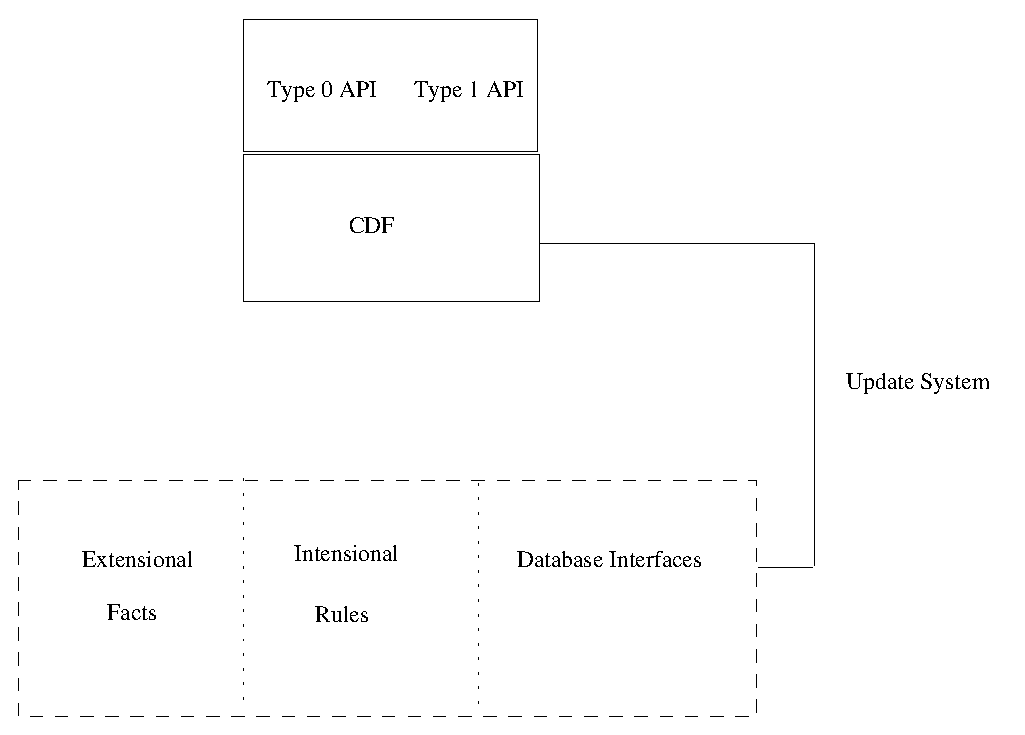
\epsfig{file=Figures/arch.eps,width=0.80\textwidth}}
\caption{A High-Level Architecture of CDF and XJ}
\label{fig:arch}
\end{figure}
%--------------

CDF instances can be classified either as Type-0 or a Type-1, each of
which has its own interface.  Type-0 instances are useful for storing
large amounts of information; and consistency and implication in
Type-0 instances is computable in polynomial time.  Type-0 instances
describe classes by existential and universal relations, qualified
number restrictions, and relational hierarchies, but descriptions omit
negation and disjunction. Type-0 instances also support a direct
product construction for objects and classes.  
\mycomment{
These product classes and objects can be useful for representing
certain types of non-binary relations, and are particularly useful for
incorporating knowledge represented as RDF facts \cite{}.  }
Information in Type-0 CDF instances is tightly coupled to XSB's
query mechanism, and CDF ensures that only the most specific answers
(according to a given inheritance hierarchy) are returned for any
Type-0 query.

Type-1 instances extend Type-0 instances to describe classes using
negation and disjunction, and thus permit descriptions that are
equivalent to an expressive description logic.  In fact, a Type-1 CDF
instance can be seen as a knowledge base in which various classes are
described via {\em class expressions}, which correspond to formulas in
description logics.  Reasoning in Type-1 instances is done via the CDF
theorem-prover.  Using the Type-1 API, users may ask whether a given
class or object is consistent, whether a given class expression is
consistent with a class or object; or whether a given class expression
is entailed by a given class or object.  The problems of determining
consistency or entailment of a Type-1 class expression have a high
degree of complexity.  To solve these problems the CDF theorem prover
uses several heuristics, but a determined (or unlucky) user can always
find class expressions that require a large amount of time to check.

Of course, ontology management systems require many features in
addition to reasoning and representation features \cite{MGPS03}.  We
mention some of these features.

\begin{itemize}
\item {\em A Semantic Checking System}.  CDF has various mechanisms for
ensuring consistency of objects and classes both at the Type-0 or
Type-1 level.  Various levels of consistency can be checked during
various operations on the CDF instance.
%
\item {\em A Component System}. Reusability of ontologies is supported
by the {\em component} structure of CDF.  An ontology component may be
maintained by separate users or organizations in different locations
and assembled in various ways by applications.
%
\item {\em A Concurrency System}. (Non open-source) Based on the
component structure, the {\em concurrency} mechanism for CDF allows
users to update their own CDF instances and to periodically update a
common store. Naturally, the various mechanisms in CDF for ensuring
consistency that are vital to ensuring coherency when users update
their systems concurrently.
%
\item {\em Database Interfaces}. (Non open-souce) CDF supports various
interfaces to databases so that CDF facts can be stored in a database
or mapped to database tables.
\end{itemize}

Based on these features, CDF can support user interfaces in a number
of ways.  One of the most convenient is to use a XSB/Java interface
such as InterProlog~\cite{Cale01} or JAXSB~(see
\texttt{http://xsb.sourceforge.net}) and then write a user interface in
Swing or some other Java Graphics library.  One of the easiest ways to
do this is to make use of the {\em XJ system} which allows Swing Gui
objects to be represented as Prolog terms (the XJ system is non
open-source) From a systems perspective, a graphical interface is then
written XJ library Swing widgets or specialized XJ-CDF Swing widgets.
CDF per-se has the following graphical packages and applications.
%
\begin{itemize}
%
\item {\em An XJ Caching System}. Adds and deletes to CDF are extended
with a notification mechanism so that Java Swing objects (created with
XJ, XSB's graphics system) reflect the state of CDF even when it
dynamically changes.
%
\item {\em A Visual Editor}. Finally,  CDF supports a graphical editor
that allows users both to visualize an ontology and to perform the
functions mentioned so far.
\end{itemize}
%
Extensional facts, intensional rules, updates, the Type-0 and Type-1
interfaces, consistency checking predicates and the full component
system are available as an open-source package for XSB.  Other
features, concurrency mechanisms, specialized database interfaces, XJ
support and the editor are not open-source.  The open-source code can
be obtained via \texttt{xsb.sourceforge.net}.  Inquiries about the full
Coherent Description System should be made to
\texttt{ode@xsb.com}.




    \chapter{Installation}
        
\section{Getting TPG}

TPG is freely available on its web page (\url{http://cdsoft.fr/tpg}). It is distributed as a package using \emph{distutils}\footnote{distutils is a Python package used to distribute Python softwares}.

\section{Requirements}

TPG is a \emph{pure Python} package.
It may run on \emph{any platform} supported by Python.
The only requirement of TPG is \emph{Python~2.2} or newer (\emph{Python~3.2} is also supported). Python can be downloaded at \url{http://www.python.org}.

\section{TPG for Linux and other Unix like}                 \label{linux_install}

Download \mbox{\emph{TPG-X.Y.Z.tar.gz}}, unpack and run the installation program:
\begin{quote}
\begin{verbatim}
    tar xzf TPG-X.Y.Z.tar.gz
    cd TPG-X.Y.Z
    python setup.py install
\end{verbatim}
\end{quote}
You may need to be logged as root to install TPG.

\section{TPG for other operating systems}

TPG should run on any system provided that Python is installed. You should be able to install it by running the \mbox{\emph{setup.py}} script (see~\ref{linux_install}).

    \chapter{Tutorial}                                      \label{tpg:tutorial}
        \section{Introduction}

This short tutorial shows how to make a simple calculator.
The calculator will compute basic mathematical expressions (\verb|+, -, *, /|) possibly nested in parenthesis.
We assume the reader is familiar with regular expressions.

\section{Defining the grammar}

Expressions are defined with a grammar.
For example an expression is a sum of terms and a term is a product of factors. A factor is either a number or a complete expression in parenthesis.

We describe such grammars with rules. A rule describe the composition of an item of the language. In our grammar we have 3 items (Expr, Term, Factor). We will call these items `symbols' or `non terminal symbols'. The decomposition of a symbol is symbolized with $\to$.
The grammar of this tutorial is given in figure~\ref{tut:gramsymb_calc}.

\begin{tableau}
\caption{Grammar for expressions}                           \label{tut:gramsymb_calc}
\begin{tabular}{| l | p{7cm} |}
\hline
    Grammar rule & Description \\
\hline
\hline
    $Expr~\to~Term~(('+'|'-')~Term)*$
        & An expression is a term eventually followed with a plus ($'+'$) or a minus ($'-'$) sign and an other term any number of times ($*$ is a repetition of an expression 0 or more times). \\
\hline
    $Term~\to~Fact~(('*'|'/')~Fact)*$
        & A term is a factor eventually followed with a $'*'$ or $'/'$ sign and an other factor any number of times. \\
\hline
    $Fact~\to~number~|~'('~Expr~')'$
        & A factor is either a number or an expression in parenthesis. \\
\hline
\end{tabular}
\end{tableau}

We have defined here the grammar rules (i.e. the sentences of the language). We now need to describe the lexical items (i.e. the words of the language). These words - also called \emph{terminal symbols} - are described using regular expressions. In the rules we have written some of these terminal symbols ($+, -, *, /, (, )$). We have to define \emph{number}. For sake of simplicity numbers are integers composed of digits (the corresponding regular expression can be $[0-9]+$).
To simplify the grammar and then the Python script we define two terminal symbols to group the operators (additive and multiplicative operators). We can also define a special symbol that is ignored by TPG. This symbol is used as a separator. This is generaly usefull for white spaces and comments. The terminal symbols are given in figure~\ref{tut:token_calc}

\begin{tableau}
\caption{Terminal symbol definition for expressions}        \label{tut:token_calc}
\begin{tabular}{| l | l | l |}
\hline
    Terminal symbol & Regular expression & Comment \\
\hline
\hline
    number & $[0-9]+$ or $\backslash d+$ & One or more digits \\
\hline
    add & $[+-]$ & a $+$ or a $-$ \\
\hline
    mul & $[*/]$ & a $*$ or a $/$ \\
\hline
    spaces & $\backslash s+$ & One or more spaces \\
\hline
\end{tabular}
\end{tableau}

This is sufficient to define our parser with TPG. The grammar of the expressions in TPG can be found in figure~\ref{tut:recognizer}.

\begin{code}
\caption{Grammar of the expression recognizer}              \label{tut:recognizer}
\begin{verbatimtab}[4]
class Calc(tpg.Parser):
    r"""

    separator spaces: '\s+' ;
    token number: '\d+' ;
    token add: '[+-]' ;
    token mul: '[*/]' ;

    START -> Expr ;

    Expr -> Term ( add Term )* ;

    Term -> Fact ( mul Fact )* ;

    Fact -> number | '\(' Expr '\)' ;

    """
\end{verbatimtab}
\end{code}

\emph{Calc} is the name of the Python class generated by TPG. \emph{START} is a special non terminal symbol treated as the \emph{axiom}\footnote{The axiom is the symbol from which the parsing starts} of the grammar.

With this small grammar we can only recognize a correct expression. We will see in the next sections how to read the actual expression and to compute its value.

\section{Reading the input and returning values}

The input of the grammar is a string. To do something useful we need to read this string in order to transform it into an expected result.

This string can be read by catching the return value of terminal symbols. By default any terminal symbol returns a string containing the current token. So the token $'\backslash('$ always returns the string $'('$. For some tokens it may be useful to compute a Python object from the token. For example \emph{number} should return an integer instead of a string, \emph{add} and \emph{mul} should return a function corresponding to the operator. That why we will add a function to the token definitions. So we associate \emph{int} to \emph{number} and \emph{make\_op} to \emph{add} and \emph{mul}.

\emph{int} is a Python function converting objects to integers and \emph{make\_op} is a user defined function (figure~\ref{tut:make_op}).

\begin{code}
\caption{\emph{make\_op} function}                          \label{tut:make_op}
\begin{verbatimtab}[4]
def make_op(s):
    return {
        '+': lambda x,y: x+y,
        '-': lambda x,y: x-y,
        '*': lambda x,y: x*y,
        '/': lambda x,y: x/y,
    }[s]
\end{verbatimtab}
\end{code}

To associate a function to a token it must be added after the token definition as in figure~\ref{tut:tokens}

\begin{code}
\caption{Token definitions with functions}                  \label{tut:tokens}
\begin{verbatimtab}[4]
    separator spaces: '\s+' ;
    token number: '\d+' int ;
    token add: '[+-]' make_op;
    token mul: '[*/]' make_op;
\end{verbatimtab}
\end{code}

We have specified the value returned by the token. To read this value after a terminal symbol is recognized we will store it in a Python variable. For example to save a \emph{number} in a variable \emph{n} we write \emph{number/n}.
In fact terminal and non terminal symbols can return a value. The syntax is the same for both sort of symbols. In non terminal symbol definitions the return value defined at the left hand side is the expression return by the symbol. The return values defined in the right hand side are just variables to which values are saved. A small example may be easier to understand (figure~\ref{tut:ret_val}).

\begin{tableau}
\caption{Return values for (non) terminal symbols}          \label{tut:ret_val}
\begin{tabular}{| l | p{9cm} |}
\hline
    Rule & Comment \\
\hline
    \verb!X/x ->!           & Defines a symbol \emph{X}. When \emph{X} is called, \emph{x} is returned. \\
    \verb!Y/y!              & \emph{X} starts with a \emph{Y}. The return value of \emph{Y} is saved in \emph{y}. \\
    \verb!Z/z!              & The return value of \emph{Z} is saved in \emph{z}. \\
    \verb!$ x = y+z $!      & Computes \emph{x}. \\
    \verb!;!                & Returns \emph{x}. \\
\hline
\end{tabular}
\end{tableau}

In the example described in this tutorial the computation of a \emph{Term} is made by applying the operator to the factors, this value is then returned:

\begin{verbatimtab}[4]
    Expr/t -> Term/t ( add/op Term/f $t=op(t,f)$ )* ;
\end{verbatimtab}

This example shows how to include Python code in a rule. Here \verb!$...$! is copied verbatim in the generated parser.

Finally the complete parser is given in figure~\ref{tut:parser}.

\begin{code}
\caption{Expression recognizer and evaluator}               \label{tut:parser}
\begin{verbatimtab}[4]
class Calc(tpg.Parser):
    r"""

    separator spaces: '\s+' ;

    token number: '\d+' int ;
    token add: '[+-]' make_op ;
    token mul: '[*/]' make_op ;

    START -> Expr ;

    Expr/t -> Term/t ( add/op Term/f $t=op(t,f)$ )* ;

    Term/f -> Fact/f ( mul Fact/a $f=op(f,a)$ )* ;

    Fact/a -> number/a | '\(' Expr/a '\)' ;

    """
\end{verbatimtab}
\end{code}

\section{Embeding the parser in a script}

Since TPG 3 embeding parsers in a script is very easy since the grammar is the doc string\footnote{It may be a good pratice to use only raw strings. This will ease the pain of writing regular expressions.} of a class (see figure~\ref{tut:build_scheme}).

\begin{code}
\caption{Writting TPG grammars in Python}             \label{tut:build_scheme}
\begin{verbatimtab}[4]
import tpg

class MyParser(tpg.Parser):
    r""" # Your grammar here """

# You can instanciate your parser here
my_parser = MyParser()
\end{verbatimtab}
\end{code}

To use this parser you now just need to instanciate an object of the class \emph{Calc} as in figure~\ref{tut:calc}.

\begin{code}
\caption{Complete Python script with expression parser}     \label{tut:calc}
\begin{verbatimtab}[4]
import tpg

def make_op(s):
    return {
        '+': lambda x,y: x+y,
        '-': lambda x,y: x-y,
        '*': lambda x,y: x*y,
        '/': lambda x,y: x/y,
    }[s]

class Calc(tpg.Parser):
    r"""

    separator spaces: '\s+' ;

    token number: '\d+' int ;
    token add: '[+-]' make_op ;
    token mul: '[*/]' make_op ;

    START/e -> Term/e ;
    Term/t -> Fact/t ( add/op Fact/f $t=op(t,f)$ )* ;
    Fact/f -> Atom/f ( mul/op Atom/a $f=op(f,a)$ )* ;
    Atom/a -> number/a | '\(' Term/a '\)' ;

    """

calc = Calc()
expr = raw_input('Enter an expression: ')
print expr, '=', calc(expr)
\end{verbatimtab}
\end{code}

\clearpage

\section{Conclusion}

This tutorial shows some of the possibilities of TPG.
If you have read it carefully you may be able to start with TPG.
The next chapters present TPG more precisely.
They contain more examples to illustrate all the features of TPG.

Happy TPG'ing!


\cleardoublepage
\part{TPG reference}                                        \label{tpg:core}
    \chapter{Usage}
        \section{Package content}

TPG is a package which main function is to define a class which particular metaclass converts a doc string into a parser.
You only need to import TPG and use these five objects:

\begin{description}
    \item [tpg.Parser:]
        This is the base class of the parsers you want to define.
    \item [tpg.Error:]
        This exception is the base of all TPG exceptions.
    \item [tpg.LexicalError:]
        This exception is raised when the lexer fails.
    \item [tpg.SyntacticError:]
        This exception is raised when the parser fails.
    \item [tpg.SemanticError:]
        This exception is raised by the grammar itself
        when some semantic properties fail.
\end{description}

The grammar must be in the doc string of the class (see figure~\ref{usage:embed}).

\begin{code}
\caption{Grammar embeding example}                          \label{usage:embed}
\begin{verbatimtab}[4]
    class Foo(tpg.Parser):
        r"""

        START/x -> Bar/x ;

        Bar/x -> 'bar'/x ;

        """
\end{verbatimtab}
\end{code}

Then you can use the new generated parser. The parser is simply a Python class (see figure~\ref{usage:inst}).

\begin{code}
\caption{Parser usage example}                              \label{usage:inst}
\begin{verbatimtab}[4]
    test = "bar"
    my_parser = Foo()
    x = my_parser(test)               # Uses the START symbol
    print x
    x = my_parser.parse('Bar', test)  # Uses the Bar symbol
    print x
\end{verbatimtab}
\end{code}

\section{Command line usage}

The \emph{tpg} script reads a Python script and replaces TPG grammars (in doc string) by Python code.
To produce a Python script (*.py) from a script containing grammars (*.pyg) you can use \emph{tpg} as follow:

\begin{verbatimtab}[4]
    tpg [-v|-vv] grammar.pyg [-o parser.py]
\end{verbatimtab}

\emph{tpg} accepts some options on the command line:

\begin{description}
    \item [-v] turns \emph{tpg} into a verbose mode (it displays parser names).
    \item [-vv] turns \emph{tpg} into a more verbose mode (it displays parser names and simplified rules).
    \item [-o file.py] tells \emph{tpg} to generate the parser in \emph{file.py}. The default output file is \emph{grammar.py} if -o option is not provided and \emph{grammar.pyg} is the name of the grammar.
\end{description}

Notice that .pyg files are valid Python scripts. So you can choose the run .pyg file (slower startup but easier for debugging purpose) or turn them into a .py file (faster startup but needs a "precompilation" stage).
You can also write .py scripts containing grammars to be used as Python scripts.

In fact I only use the \emph{tpg} script to convert \emph{tpg.pyg} into \emph{tpg.py} because TPG needs obviously to be a pure Python script (it can not translate itself at runtime). Then in most cases it is very convenient to directly write grammars in Python scripts.


    \chapter{Grammar structure}
        \section{TPG grammar structure}

TPG grammars are contained in the doc string\footnote{If the grammar (i.e. the doc string) is a unicode string then the generated parser can parse unicode strings} of the parser class.
TPG grammars may contain three parts:

\begin{description}
    \item [ReStructuredText docstring]
        is a part of the grammar that is ignored by TPG. It shall end with a `::` at the end of a line.
    \item [Options]
        are defined at the beginning of the grammar (see~\ref{grammar:options}).
    \item [Tokens]
        are introduced by the \emph{token} or \emph{separator} keyword (see~\ref{lexer:token_def}).
    \item [Rules]
        are described after tokens (see~\ref{grammar:parser}).
\end{description}

See figure~\ref{grammar:struct} for a generic TPG grammar.

\begin{code}
\caption{TPG grammar structure}                             \label{grammar:struct}
\begin{verbatimtab}[4]
class Foo(tpg.Parser):
    r"""
    Here is some ReStructuredText documentation
    (for Sphinx for instance).

    And now, the grammar::

        # Options
        set lexer = CSL

        # Tokens
        separator spaces    '\s+'       ;
        token int           '\d+'   int ;

        # Rules
        START -> X Y Z ;

    """

foo = Foo()
result = foo("input string")
\end{verbatimtab}
\end{code}

\section{Comments}

Comments in TPG start with \emph{\#} and run until the end of the line.

\begin{verbatimtab}[4]
    # This is a comment
\end{verbatimtab}

\section{Options}                                           \label{grammar:options}

Some options can be set at the beginning of TPG grammars.
The syntax for options is:

\begin{description}
    \item [set \emph{name} = \emph{$value$}] sets the \emph{name} option to \emph{$value$}.
\end{description}

\subsection{Lexer option}                                   \label{grammar:lexer_option}

The \emph{lexer} option tells TPG which lexer to use.

\begin{description}
    \item [set lexer = NamedGroupLexer] is the default lexer.
        It is context free and uses named groups of the \emph{re} package (and its limitation of 100 named groups, ie 100 tokens).
    \item [set lexer = Lexer] is similar to \emph{NamedGroupLexer} but doesn't use named groups.
        It is slower than \emph{NamedGroupLexer}.
    \item [set lexer = CacheNamedGroupLexer] is similar to \emph{NamedGroupLexer} except that tokens are first stored in a list.
        It is faster for heavy backtracking grammars.
    \item [set lexer = CacheLexer] is similar to \emph{Lexer} except that tokens are first stored in a list.
        It is faster for heavy backtracking grammars.
    \item [set lexer = ContextSensitiveLexer] is the context sensitive lexer (see~\ref{tpg:CSL}).
\end{description}

\subsection{Word bondary option}                            \label{grammar:word_boundary_option}

The \emph{word\_boundary} option tells the lexer to search for word boundaries after identifiers.

\begin{description}
    \item [set word\_boundary = True] enables the word boundary search. This is the default.
    \item [set word\_boundary = False] disables the word boundary search.
\end{description}

\subsection{Regular expression options}

The \emph{re} module accepts some options to define the behaviour of the compiled regular expressions.
These options can be changed for each parser.

\begin{description}
    \item [set lexer\_ignorecase = True] enables the \emph{re.IGNORECASE} option.
    \item [set lexer\_locale = True] enables the \emph{re.LOCALE} option.
    \item [set lexer\_multiline = True] enables the \emph{re.MULTILINE} option.
    \item [set lexer\_dotall = True] enables the \emph{re.DOTALL} option.
    \item [set lexer\_verbose = True] enables the \emph{re.VERBOSE} option.
    \item [set lexer\_unicode = True] enables the \emph{re.UNICODE} option.
\end{description}

\section{Python code}                                       \label{grammar:code}

Python code sections are not handled by TPG.
TPG won't complain about syntax errors in Python code sections, it is Python's job.
They are copied verbatim to the generated Python parser.

\subsection{Syntax}

Before TPG 3, Python code was enclosed in double curly brackets.
That means that Python code must not contain two consecutive close brackets.
You can avoid this by writting \emph{\}~\}} (with a space) instead of \emph{\}\}} (without space).
This syntaxe is still available but the new syntax may be more readable.
The new syntax uses \emph{\$} to delimit code sections.
When several \emph{\$} sections are consecutive they are seen as a single section.

\subsection{Indentation}

Python code can appear in several parts of a grammar.
Since indentation has a special meaning in Python it is important to know how TPG handles spaces and tabulations at the beginning of the lines.

When TPG encounters some Python code it removes from all non blank lines the spaces and tabulations that are common to every lines.
TPG considers spaces and tabulations as the same character so it is important to always use the same indentation style.
Thus it is advised not to mix spaces and tabulations in indentation.
Then this code will be reindented when generated according to its location (in a class, in a method or in global space).

The figure~\ref{grammar:indent} shows how TPG handles indentation.

\begin{tableau}
\caption{Code indentation examples}                         \label{grammar:indent}
\begin{tabular}{| p{3.5cm} | p{3.5cm} | p{3cm} | p{3cm} |}
\hline
    Code in grammars (old syntax) & Code in grammars (new syntax) & Generated code & Comment \\
\hline
\hline

    \begin{verbatim*}
{{
    if 1==2:
        print "???"
    else:
        print "OK"
}}
    \end{verbatim*}
    &
    \begin{verbatim*}

$  if 1==2:
$      print "???"
$  else:
$      print "OK"

    \end{verbatim*}
    &
    \begin{verbatim*}

if 1==2:
    print "???"
else:
    print "OK"
    \end{verbatim*}
    &
    \emph{Correct}: these lines have four spaces in common.  These spaces are removed.
    \\

\hline

    \begin{verbatim*}
{{  if 1==2:
        print "???"
    else:
        print "OK"
}}
    \end{verbatim*}
    &
The new syntax has no trouble in that case.
    &
    \begin{verbatim*}
if 1==2:
      print "???"
  else:
      print "OK"
    \end{verbatim*}
    &
    \emph{WRONG}: it is a bad idea to start a multiline code section on the first line since the common indentation may be different from what you expect.  No error will be raised by TPG but Python will not compile this code.
    \\

\hline

    \begin{verbatim*}
{{    print "OK" }}
    \end{verbatim*}
    &
    \begin{verbatim*}
$       print "OK"
    \end{verbatim*}
or
    \begin{verbatim*}
$ print "OK" $
    \end{verbatim*}
    &
    \begin{verbatim*}
print "OK"
    \end{verbatim*}
    &
    \emph{Correct}: indentation does not matter in a one line Python code.
    \\

\hline

\end{tabular}
\end{tableau}

\section{TPG parsers}                                       \label{grammar:parser}

TPG parsers are \emph{tpg.Parser} classes.
The grammar is the doc string of the class.

\subsection{Methods}

As TPG parsers are just Python classes, you can use them as normal classes.
If you redefine the \emph{\_\_init\_\_} method, do not forget to call \emph{tpg.Parser.\_\_init\_\_}.

\subsection{Rules}

Each rule will be translated into a method of the parser.


    \chapter{Lexer}
        \section{Regular expression syntax}

The lexer is based on the \emph{re}\footnote{\emph{re} is a standard Python module. It handles regular expressions. For further information about \emph{re} you can read \url{http://docs.python.org/lib/module-re.html}} module.
TPG profits from the power of Python regular expressions.
This document assumes the reader is familiar with regular expressions.

You can use the syntax of regular expressions as expected by the \emph{re} module except from the grouping by name syntax since it is used by TPG to decide which token is recognized.

Here is a summary\footnote{From the Python documentation: \url{http://docs.python.org/lib/re-syntax.html}} of the regular expression syntax:

\begin{description}
    \item ["."]
    (Dot.) In the default mode, this matches any character except a newline. If the \emph{DOTALL} flag has been specified, this matches any character including a newline.
    \item ["$\hat{~}$"]
    (Caret.) Matches the start of the string, and in \emph{MULTILINE} mode also matches immediately after each newline.
    \item ["\$"]
    Matches the end of the string or just before the newline at the end of the string, and in \emph{MULTILINE} mode also matches before a newline. $foo$ matches both 'foo' and 'foobar', while the regular expression $foo\$$ matches only 'foo'. More interestingly, searching for $foo.\$$ in 'foo1$\backslash$nfoo2$\backslash$n' matches 'foo2' normally, but 'foo1' in \emph{MULTILINE} mode.
    \item ["*"]
    Causes the resulting RE to match 0 or more repetitions of the preceding RE, as many repetitions as are possible. $ab*$ will match 'a', 'ab', or 'a' followed by any number of 'b's.
    \item ["+"]
    Causes the resulting RE to match 1 or more repetitions of the preceding RE. $ab+$ will match 'a' followed by any non-zero number of 'b's; it will not match just 'a'.
    \item ["?"]
    Causes the resulting RE to match 0 or 1 repetitions of the preceding RE. $ab?$ will match either 'a' or 'ab'.
    \item [*?, +?, ??]
    The "*", "+", and "?" qualifiers are all greedy; they match as much text as possible. Sometimes this behaviour isn't desired; if the RE $<.*>$ is matched against '$<$H1$>$title$<$/H1$>$', it will match the entire string, and not just '$<$H1$>$'. Adding "?" after the qualifier makes it perform the match in non-greedy or minimal fashion; as few characters as possible will be matched. Using $.*?$ in the previous expression will match only '$<$H1$>$'.
    \item [$\{$m$\}$]
    Specifies that exactly m copies of the previous RE should be matched; fewer matches cause the entire RE not to match. For example, $a\{6\}$ will match exactly six "a" characters, but not five.
    \item [$\{$m,n$\}$]
    Causes the resulting RE to match from m to n repetitions of the preceding RE, attempting to match as many repetitions as possible. For example, $a\{3,5\}$ will match from 3 to 5 "a" characters. Omitting m specifies a lower bound of zero, and omitting n specifies an infinite upper bound. As an example, $a\{4,\}b$ will match aaaab or a thousand "a" characters followed by a b, but not aaab. The comma may not be omitted or the modifier would be confused with the previously described form.
    \item [\{m,n\}?]
    Causes the resulting RE to match from m to n repetitions of the preceding RE, attempting to match as few repetitions as possible. This is the non-greedy version of the previous qualifier. For example, on the 6-character string 'aaaaaa', $a\{3,5\}$ will match 5 "a" characters, while $a\{3,5\}?$ will only match 3 characters.
    \item ["$\backslash$"]
    Either escapes special characters (permitting you to match characters like "*", "?", and so forth), or signals a special sequence; special sequences are discussed below.
    \item [$\lbrack\rbrack$]
    Used to indicate a set of characters. Characters can be listed individually, or a range of characters can be indicated by giving two characters and separating them by a "-". Special characters are not active inside sets. For example, $[akm\$]$ will match any of the characters "a", "k", "m", or "\$"; $[a-z]$ will match any lowercase letter, and $[a-zA-Z0-9]$ matches any letter or digit. Character classes such as $\backslash$w or $\backslash$S (defined below) are also acceptable inside a range. If you want to include a "$]$" or a "-" inside a set, precede it with a backslash, or place it as the first character. The pattern $[]]$ will match '$]$', for example.

    You can match the characters not within a range by complementing the set. This is indicated by including a "$\hat{~}$" as the first character of the set; "$\hat{~}$" elsewhere will simply match the "$\hat{~}$" character. For example, $[\hat{~}5]$ will match any character except "5", and $[\hat{~}\hat{~}]$ will match any character except "$\hat{~}$".
    \item ["$\vert$"]
    $A|B$, where $A$ and $B$ can be arbitrary REs, creates a regular expression that will match either A or B. An arbitrary number of REs can be separated by the "$\vert$" in this way. This can be used inside groups (see below) as well. As the target string is scanned, REs separated by "$\vert$" are tried from left to right. When one pattern completely matches, that branch is accepted. This means that once A matches, B will not be tested further, even if it would produce a longer overall match. In other words, the "$|$" operator is never greedy. To match a literal "$|$", use $\backslash|$, or enclose it inside a character class, as in $[|]$.
    \item [(...)]
    Matches whatever regular expression is inside the parentheses, and indicates the start and end of a group; the contents of a group can be retrieved after a match has been performed, and can be matched later in the string with the $\backslash number$ special sequence, described below. To match the literals "(" or ")", use $\backslash($ or $\backslash)$, or enclose them inside a character class: $[(]$ $[)]$.
    \item [(?=...)]
    Matches if ... matches next, but doesn't consume any of the string. This is called a lookahead assertion. For example, $Isaac (?=Asimov)$ will match 'Isaac ' only if it's followed by 'Asimov'.
    \item [(?!...)]
    Matches if ... doesn't match next. This is a negative lookahead assertion. For example, $Isaac (?!Asimov)$ will match 'Isaac ' only if it's not followed by 'Asimov'.
    \item [(?$<$=...)]
    Matches if the current position in the string is preceded by a match for ... that ends at the current position. This is called a positive lookbehind assertion. $(?<=abc)def$ will find a match in "abcdef", since the lookbehind will back up 3 characters and check if the contained pattern matches. The contained pattern must only match strings of some fixed length, meaning that $abc$ or $a|b$ are allowed, but $a*$ and $a\{3,4\}$ are not.
    \item [(?$<$!...)]
    Matches if the current position in the string is not preceded by a match for .... This is called a negative lookbehind assertion. Similar to positive lookbehind assertions, the contained pattern must only match strings of some fixed length. Patterns which start with negative lookbehind assertions may match at the beginning of the string being searched.
    \item [$\backslash A$]
    Matches only at the start of the string.
    \item [$\backslash b$]
    Matches the empty string, but only at the beginning or end of a word. A word is defined as a sequence of alphanumeric or underscore characters, so the end of a word is indicated by whitespace or a non-alphanumeric, non-underscore character. Note that $\backslash b$ is defined as the boundary between $\backslash w$ and $\backslash W$, so the precise set of characters deemed to be alphanumeric depends on the values of the UNICODE and LOCALE flags. Inside a character range, $\backslash b$ represents the backspace character, for compatibility with Python's string literals.
    \item [$\backslash B$]
    Matches the empty string, but only when it is not at the beginning or end of a word. This is just the opposite of $\backslash b$, so is also subject to the settings of LOCALE and UNICODE.
    \item [$\backslash d$]
    Matches any decimal digit; this is equivalent to the set $[0-9]$.
    \item [$\backslash D$]
    Matches any non-digit character; this is equivalent to the set $[\hat{~}0-9]$.
    \item [$\backslash s$]
    Matches any whitespace character; this is equivalent to the set $[~\backslash t\backslash n\backslash r\backslash f\backslash v]$.
    \item [$\backslash S$]
    Matches any non-whitespace character; this is equivalent to the set $[\hat{~}~\backslash t\backslash n\backslash r\backslash f\backslash v]$.
    \item [$\backslash w$]
    When the LOCALE and UNICODE flags are not specified, matches any alphanumeric character and the underscore; this is equivalent to the set $[a-zA-Z0-9\_]$. With LOCALE, it will match the set $[0-9\_]$ plus whatever characters are defined as alphanumeric for the current locale. If UNICODE is set, this will match the characters $[0-9\_]$ plus whatever is classified as alphanumeric in the Unicode character properties database.
    \item [$\backslash W$]
    When the LOCALE and UNICODE flags are not specified, matches any non-alphanumeric character; this is equivalent to the set $[\hat{~}a-zA-Z0-9\_]$. With LOCALE, it will match any character not in the set $[0-9\_]$, and not defined as alphanumeric for the current locale. If UNICODE is set, this will match anything other than $[0-9\_]$ and characters marked as alphanumeric in the Unicode character properties database.
    \item [$\backslash Z$]
    Matches only at the end of the string.
    \item [$\backslash a ~ \backslash f ~ \backslash n ~ \backslash r ~ \backslash t ~ \backslash v ~ \backslash x ~ \backslash\backslash$]
    Most of the standard escapes supported by Python string literals are also accepted by the regular expression parser.
    \item [$\backslash 0xyz$, $\backslash xyz$] Octal escapes are included in a limited form: If the first digit is a 0, or if there are three octal digits, it is considered an octal escape. As for string literals, octal escapes are always at most three digits in length.
\end{description}

\section{Token definition}                                  \label{lexer:token_def}

\subsection{Predefined tokens}

Tokens can be explicitely defined by the \emph{token} and \emph{separator} keywords.

A token is defined by:

\begin{description}
    \item [a name] which identifies the token.
        This name is used by the parser.
    \item [a regular expression] which describes what to match to recognize the token.
    \item [an action] which can translate the matched text into a Python object. It can be a function of one argument or a non callable object. If it is not callable, it will be returned for each token otherwise it will be applied to the text of the token and the result will be returned. This action is optional. By default the token text is returned.
\end{description}

Token definitions must end with a \emph{;} when no action is specified. The dots after the token name are optional.

See figure~\ref{lexer:tokens} for examples.

\begin{code}
\caption{Token definition examples}                         \label{lexer:tokens}
\begin{verbatimtab}[4]
    #     name     reg. exp        action
    token integer: '\d+'           int;
    token ident  : '[a-zA-Z]\w*'   ;
    token bool   : 'True|False'    $ lambda b: b=='True'

    separator spaces  : '\s+';     # white spaces
    separator comments: '#.*';     # comments
\end{verbatimtab}
\end{code}

The order of the declaration of the tokens is important. The first token that is matched is returned. The regular expression has a special treatment. If it describes a keyword, TPG also looks for a word boundary after the keyword. If you try to match the keywords \emph{if} and \emph{ifxyz} TPG will internally search \verb$if\b$ and \verb$ifxyz\b$. This way, \emph{if} won't match \emph{ifxyz} and won't interfere with general identifiers (\verb$\w+$ for example). This behaviour can be disabled since the version 3 of TPG (see~\ref{grammar:word_boundary_option}).

There are two kinds of tokens. Tokens defined by the \emph{token} keyword are parsed by the parser and tokens defined by the \emph{separator} keyword are considered as separators (white spaces or comments for example) and are wiped out by the lexer.

\subsection{Inline tokens}

Tokens can also be defined on the fly. Their definitions are then inlined in the grammar rules.
This feature may be useful for keywords or punctuation signs.
Inline tokens can not be transformed by an action as predefined tokens.
They always return the token in a string.

See figure~\ref{lexer:inline_tokens} for examples.

\begin{code}
\caption{Inline token definition examples}                  \label{lexer:inline_tokens}
\begin{verbatimtab}[4]
    IfThenElse ->
        'if' Cond
        'then' Statement
        'else' Statement
        ;
\end{verbatimtab}
\end{code}

Inline tokens have a higher precedence than predefined tokens to avoid conflicts (an inlined \emph{if} will not be matched as a predefined \emph{identifier}).

\section{Token matching}                                    \label{lexer:token_matching}

TPG works in two stages.
The lexer first splits the input string into a list of tokens and then the parser parses this list.
The default lexer is lazy in TPG 3. Tokens are generated while parsing.
This way TPG 3 need less memory when parsing huge files.

\subsection{Splitting the input string}

The lexer splits the input string according to the token definitions (see~\ref{lexer:token_def}). When the input string can not be matched a \emph{tpg.LexicalError} exception is raised.

The lexer may loop indefinitely if a token can match an empty string since empty strings are everywhere.

\subsection{Matching tokens in grammar rules}

Tokens are matched as symbols are recognized.
Predefined tokens have the same syntax than non terminal symbols.
The token text (or the result of the function associated to the token) can be saved by the infix \emph{/} operator (see figure~\ref{lexer:token_ret_val}).

\begin{code}
\caption{Token usage examples}                              \label{lexer:token_ret_val}
\begin{verbatimtab}[4]
    S -> ident/i;
\end{verbatimtab}
\end{code}

Inline tokens have a similar syntax. You just write the regular expression (in a string). Its text can also be saved (see figure~\ref{lexer:inline_token_ret_val}).

\begin{code}
\caption{Token usage examples}                              \label{lexer:inline_token_ret_val}
\begin{verbatimtab}[4]
    S -> '\(' '\w+'/i '\)';
\end{verbatimtab}
\end{code}

%\section{Special tokens}                                    \label{lexer:special_tokens}
%
%Their are some special tokens that have been requested by some users but these tokens can not be easily
%described by TPG using classical token definition (see~\ref{lexer:token_def}).
%
%\subsection{Indent and deindent tokens}                     \label{lexer:indent_deindent}
%
%TPG is written in Python so is should be easy to handle INDENT and DEDENT tokens as in Python language.
%These tokens are introduced in the source to be parsed by a preprocessor, before the lexer is activated.
%Spaces in the beginning the lines are replaced by indent and deindent tokens when needed.
%These special tokens are characters which ASCII codes are 16 and 17.
%These characters may not be used in regular text files.
%
%\subsubsection{Indent definition}
%
%The \emph{indent} option (see~\ref{grammar:options}) has been added to define the indentation.
%It has two values.
%The first one is a regular expression describing the indentation, usually spaces and tabulations.
%The second one is a regular expression describing the lines not to be taken into account, usually comments.
%This second parameter describes the beginning of the line, i.e. \emph{"\#"} will match lines starting
%with a \emph{\#}.
%
%\begin{code}
%\caption{Indent and deindent definition example}            \label{lexer:indent_definition}
%\begin{verbatimtab}[4]
%    set indent = "\s", "#"
%\end{verbatimtab}
%\end{code}
%
%\subsubsection{Indent and deindent usage}                   \label{lexer:indent_usage}
%
%When the \emph{indent} option is active, \emph{indent} and \emph{deindent} tokens are defined.
%They can be used as any other token.
%
%\begin{code}
%\caption{Indent and deindent example}            \label{lexer:indent_example}
%\begin{verbatimtab}[4]
%parser IndentParser:
%
%    set indent = "\s", "#"
%
%    BLOCK ->
%        (   INSTR
%        |   indent
%                BLOCK
%            deindent
%        )*;
%\end{verbatimtab}
%\end{code}

    \chapter{Parser}
        \section{Declaration}

A parser is declared as a \emph{tpg.Parser} class.
The doc string of the class contains the definition of the tokens and rules.

\section{Grammar rules}                                         \label{parser:grammar_rules}

Rule declarations have two parts.
The left side declares the symbol associated to the rule, its attributes and its return value.
The right side describes the decomposition of the rule.
Both parts of the declaration are separated with an arrow (\emph{$\to$})
and the declaration ends with a \emph{;}.

The symbol defined by the rule as well as the symbols that appear in the rule can have attributes and return values.
The attribute list - if any - is given as an object list enclosed in left and right angles.
The return value - if any - is extracted by the infix \emph{/} operator.
When no return value is specified, TPG creates a variable named as the symbol.
See figure~\ref{parser:rule} for example.

\begin{code}
\caption{Rule declaration}                                      \label{parser:rule}
\begin{verbatimtab}[4]
    SYMBOL <att1, att2, att3> / return_expression_of_SYMBOL ->

        A <x, y> / ret_value_of_A

        B <y, z> / ret_value_of_B

        ;

    S1 / $f(A,B)$ ->
        A       # return value of A stored in variable A
        B       # return value of B stored in variable B
    ;

    S2 ->       # we can use S2 to compute the return value
        A       $ S2 = A
        B       $ S2 = f(S2, B)
    ;
\end{verbatimtab}
\end{code}

\section{Parsing terminal symbols}

Each time a terminal symbol is encountered in a rule, the parser compares it to the current token in the token list. If it is different the parser backtracks.

\section{Parsing non terminal symbols}                          \label{parser:nterm}

\subsection{Starting the parser}

You can start the parser from the axiom or from any other non terminal symbol.
When the parser can not parse the whole token list a \emph{tpg.SyntacticError} is raised.
The value returned by the parser is the return value of the parsed symbol.

\subsubsection{From the axiom}

The axiom is a special non terminal symbol named \emph{START}.
Parsers are callable objects.
When an instance of a parser is called, the \emph{START} rule is parsed.
The first argument of the call is the string to parse.
The other arguments of the call are given to the \emph{START} symbol.

This allows to simply write \verb!x=calc("1+1")! to parse and compute an expression if \emph{calc} is an instance of an expression parser.

\subsubsection{From another non terminal symbol}

It's also possible to start parsing from any other non terminal symbol.
TPG parsers have a method named \emph{parse}.
The first argument is the name of the symbol to start from.
The second argument is the string to parse.
The other arguments are given to the specified symbol.

For example to start parsing a \emph{Term}
you can write:
\begin{verbatimtab}[4]
    f=calc.parse('Term', "2*3")
\end{verbatimtab}

\subsection{In a rule}

To parse a non terminal symbol in a rule, TPG calls the rule corresponding to the symbol.

\section{Sequences}                                             \label{parser:sequences}

Sequences in grammar rules describe in which order symbols should appear in the input string.
For example the sequence \emph{A~B} recognizes an \emph{A} followed by a \emph{B}.
Sequences can be empty.

For example to say that a \emph{sum} is a \emph{term} \emph{plus} another \emph{term} you can write:
\begin{verbatimtab}[4]
    Sum -> Term '+' Term ;
\end{verbatimtab}

\section{Alternatives}                                          \label{parser:alternatives}

Alternatives in grammar rules describe several possible decompositions of a symbol.
The infix pipe operator (\emph{$\mid$}) is used to separate alternatives.
\emph{$A~\mid~B$} recognizes either an \emph{A} or a \emph{B}.
If both \emph{A} and \emph{B} can be matched only the first match is considered.
So the order of alternatives is very important.
If an alternative has an empty choice, it must be the last.
Empty choices in other positions will be reported as syntax errors.

For example to say that an \emph{atom} is an \emph{integer} or an \emph{expression in paranthesis}
you can write:
\begin{verbatimtab}[4]
    Atom -> integer | '\(' Expr '\)' ;
\end{verbatimtab}

\section{Repetitions}                                           \label{parser:repetitions}

Repetitions in grammar rules describe how many times an expression should be matched.

\begin{description}
    \item [A?] recognizes zero or one \emph{A}.
    \item [A*] recognizes zero or more \emph{A}.
    \item [A+] recognizes one or more \emph{A}.
    \item [A\{m,n\}] recognizes at least m and at most n \emph{A}.
\end{description}

Repetitions are greedy.
Repetitions are translated into Python loops.
Thus whatever the length of the repetitions, the Python stack will not overflow.

\section{Precedence and grouping}

The figure~\ref{parser:precedence} lists the different structures in increasing precedence order.
To override the default precedence you can group expressions with parenthesis.

\begin{tableau}
\caption{Precedence in TPG expressions}                         \label{parser:precedence}
\begin{tabular}{| l | l |}
\hline
    Structure           & Example \\
\hline
\hline
    Alternative         & $A~\mid~B$ \\
\hline
    Sequence            & $A~B$ \\
\hline
    Repetitions         & $A?$, $A*$, $A+$ \\
\hline
    Symbol and grouping & $A$ and $(~\ldots~)$ \\
\hline
\end{tabular}
\end{tableau}

\section{Actions}

Grammar rules can contain actions as Python code.
Python code is copied verbatim into the generated code and
is delimited by \verb!$...$!, \verb!$...EOL!\footnote{EOL means End Of Line} or \verb!{{...}}!.

Please be aware that indentation should obey Python indentation rules.
See the grammar description for further information (see figure~\ref{grammar:indent}).

\subsection{Abstract syntax trees}                              \label{parser:AST}

An abstract syntax tree (AST) is an abstract representation of the structure of the input.
A node of an AST is a Python object (there is no constraint about its class).
AST nodes are completely defined by the user.

The figure~\ref{parser:ASTinst} shows a node symbolizing a couple.

\begin{code}
\caption{AST example}                                           \label{parser:ASTinst}
\begin{verbatimtab}[4]

class Couple:
    def __init__(self, a, b):
        self.a = a
        self.b = b

class Foo(tpg.Parser):
    r"""
    COUPLE/$Couple(a,b)$ -> '\(' ITEM/a ',' ITEM/b '\)' ;

    # which is equivalent to
    # COUPLE/c -> '\(' ITEM/a ',' ITEM/b '\)' $ c = Couple(a,b) $ ;
    """
\end{verbatimtab}
\end{code}

\subsubsection{Creating an AST}

AST are created in Python code (see section~\ref{parser:AST}).

\subsubsection{Updating an AST}

When parsing lists for example it is useful to save all the items of the list.
In that case one can use a list and its append method (see figure~\ref{parser:ASTadd}).

\begin{code}
\caption{AST update example}                                    \label{parser:ASTadd}
\begin{verbatimtab}[4]

class ListParser(tpg.Parser):
    r"""
    LIST/l ->
        '\('                $ l = []
            ITEM/a          $ l.append(a)
            ( ',' ITEM/a    $ l.append(a)
            )*
        '\)'
        ;
    """
\end{verbatimtab}
\end{code}

\subsection{Text extraction}                                    \label{parser:mark}

TPG can extract a portion of the input string.
The idea is to put marks while parsing and then extract the text between the two marks.
This extracts the whole text between the marks, including the tokens defined as separators.

\subsection{Object}                                             \label{parser:object}

TPG 3 doesn't handle Python object as TPG 2.
Only identifiers, integers and strings are known.
Other objects must be written in Python code delimited either by \verb!$...$! or by \verb!{{...}}!.

\subsubsection{Argument lists and tuples}

An argument list is a comma separated list of objects.
\emph{Remember that arguments are enclosed in left and right angles.}

\begin{verbatimtab}[4]
    <object1, object2, object3>
\end{verbatimtab}

Argument lists and tuples have the same syntax except from the possibility to have
default arguments, argument lists and argument dictionnaries as arguments as in Python.

\begin{verbatimtab}[4]
    RULE<arg1, arg2=18, arg3=None, *other_args, **keywords> -> ;
\end{verbatimtab}

\subsubsection{Python code object}

A Python code object is a piece of Python code in double curly brackets or in dollar signs.
Python code used in an object expression must have only one line.

\begin{verbatimtab}[4]
    $ dict([ (x,x**2) for x in range(100) ]) $ # Python embeded in TPG
\end{verbatimtab}

\subsubsection{Text extraction}

Text extraction is done by the \emph{extract} method.
Marks can be put in the input string by the \emph{mark} method or the prefix \emph{\@} operator.

\begin{verbatimtab}[4]
    @beginning      # equivalent to $ beginning = self.mark()
    ...
    @end            # equivalent to $ end = self.mark()
    ...
    $ my_string = self.extract(beginning, end)
\end{verbatimtab}

\subsubsection{Getting the line and column number of a token}

The \emph{line} and \emph{column} methods return the line and column number of the current token.
If the first parameter is a mark (see~\ref{parser:mark}) the method returns the line number of the token following the mark.

\subsubsection{Backtracking}

The user can force the parser to backtrack in rule actions.
The module has a \emph{WrongToken} exception for that purpose (see figure~\ref{parser:wrongtoken}).

\begin{code}
\caption{Backtracking with \emph{WrongToken} example}           \label{parser:wrongtoken}
\begin{verbatimtab}[4]
    # NATURAL matches integers greater than 0
    NATURAL/n ->
        number/n
        $ if n<1: raise tpg.WrongToken $
        ;
\end{verbatimtab}
\end{code}

Parsers have another useful method named \emph{check} (see figure~\ref{parser:check}).
This method checks a condition.
If this condition is false then \emph{WrongToken} is called in order to backtrack.

\begin{code}
\caption{Backtracking with the \emph{check} method example}     \label{parser:check}
\begin{verbatimtab}[4]
    # NATURAL matches integers greater than 0
    NATURAL/n ->
        number/n
        $ self.check(n>=1) $
        ;
\end{verbatimtab}
\end{code}

A shortcut for the \emph{check} method is the \emph{check} keyword followed by the condition to check (see figure~\ref{parser:checkkw}).

\begin{code}
\caption{Backtracking with the \emph{check} keyword example}    \label{parser:checkkw}
\begin{verbatimtab}[4]
    # NATURAL matches integers greater than 0
    NATURAL/n ->
        number/n
        check $ n>=1 $
        ;
\end{verbatimtab}
\end{code}

\subsubsection{Error reporting}

The user can force the parser to stop and raise an exception.
The parser classes have a \emph{error} method for that purpose (see figure~\ref{parser:error_method}).
This method raises a \emph{SemanticError}.

\begin{code}
\caption{Error reporting the \emph{error} method example}   \label{parser:error_method}
\begin{verbatimtab}[4]
    # FRACT parses fractions
    FRACT/<n,d> ->
        number/n '/' number/d
        $ if d==0: self.error("Division by zero") $
        ;
\end{verbatimtab}
\end{code}

A shortcut for the \emph{error} method is the \emph{error} keyword followed by the object to give to the \emph{SemanticError} exception (see figure~\ref{parser:error_kw}).

\begin{code}
\caption{Error reporting the \emph{error} keyword example}  \label{parser:error_kw}
\begin{verbatimtab}[4]
    # FRACT parses fractions
    FRACT/<n,d> ->
        number/n '/' number/d
        ( check d | error "Division by zero" )
        ;
\end{verbatimtab}
\end{code}


    \chapter{Context sensitive lexer}                       \label{tpg:CSL}
        \section{Introduction}          \label{CSL}

Before the version 2 of TPG, lexers were context sensitive.
That means that the parser commands the lexer to match some tokens, i.e. different tokens can be matched in a same input string according to the grammar rules being used.
These lexers were very flexible but slower than context free lexers because TPG backtracking caused tokens to be matched several times.

In TPG 2, the lexer is called before the parser and produces a list of tokens from the input string.
This list is then given to the parser.
In this case when TPG backtracks the token list remains unchanged.

Since TPG 2.1.2, context sensitive lexers have been reintroduced in TPG.
By default lexers are context free but the \emph{CSL} option (see~\ref{grammar:lexer_option}) turns TPG into a context sensitive lexer.

\section{Grammar structure}

CSL grammars have the same structure than non CSL grammars (see~\ref{grammar:struct}) except from the \emph{lexer~=~CSL} option (see~\ref{grammar:lexer_option}).

\section{CSL lexers}

\subsection{Regular expression syntax}

The CSL lexer is based on the \emph{re} module.
The difference with non CSL lexers is that the given regular expression is compiled as this, without any encapsulation.

\subsection{Token matching}

In CSL parsers, tokens are matched as in non CSL parsers (see~\ref{lexer:token_matching}).

\section{CSL parsers}

There is no difference between CSL and non CSL parsers.

    \chapter{Debugging}
        \section{Introduction}          \label{debug}

When I need to debug a grammar I often add print statments to visualize the parser activity.
Now with TPG 3 it is possible to print such information automatically.

\section{Verbose parsers}

Normal parsers inherit from \emph{tpg.Parser}.
If you need a more verbose parser you can use \emph{tpg.VerboseParser} instead.
This parser prints information about the current token each time the lexer is called.
The debugging information has currently two levels of details.

\begin{description}
    \item [Level 0] displays no information.
    \item [Level 1] displays tokens only when the current token matches the expected token.
    \item [Level 2] displays tokens if the current token matches or not the expected token.
\end{description}

The level is defined by the attribute \emph{verbose}. Its default value is 1.

\begin{code}
\caption{Verbose parser example}                            \label{debug:example}
\begin{verbatimtab}[4]
class Test(tpg.VerboseParser):
    r"""

    START -> 'x' 'y' 'z' ;

    """

    verbose = 2
\end{verbatimtab}
\end{code}

The information displayed by verbose parsers has the following format:
\begin{verbatim}
[eat counter][stack depth]callers: (line,column) <current token> == <expected token>
\end{verbatim}

\begin{description}
    \item [$eat counter$] is the number of calls of the lexer.
    \item [$stack depth$] is the depth of the Python stack since the axiom.
    \item [$callers$] is the list of non terminal symbols called before the current symbol.
    \item [$(line,column)$] is the position of the current token in the input string.
    \item [$==$] means the current token matches the expected token (level 1 or 2).
    \item [$!=$] means the current token doesn't match the expected token (level 2).
\end{description}


\cleardoublepage
\part{Some examples to illustrate TPG}                      \label{tpg:examples}
    \chapter{Complete interactive calculator}
        \section{Introduction}

This chapter presents an extension of the calculator described in the tutorial (see~\ref{tpg:tutorial}).
This calculator has more functions and a memory.

\section{New functions}

\subsection{Trigonometric and other functions}

This calculator can compute some numerical functions (\emph{sin}, \emph{cos}, \emph{sqrt}, \ldots).
The \emph{make\_op} function (see figure~\ref{tut:make_op}) has been extended to return these functions.
Tokens must also be defined to scan function names.
\emph{funct1} defines the name of unary functions and \emph{funct2} defines the name of binary functions.
Finally the grammar rule of the atoms has been added a branch to parse functions.
The \emph{Function} non terminal symbol parser unary and binary functions.

\subsection{Memories}

The calculator has memories.
A memory cell is identified by a name.
For example, if the user types \emph{$pi = 4*atan(1)$}, the memory cell named \emph{pi} contains the value of \emph{$\pi$} and \emph{$cos(pi)$} returns \emph{$-1$}.

To display the content of the whole memory, the user can type \emph{vars}.

The variables are saved in a dictionnary.
In fact the parser itself is a dictionnary (the parser inherits from the \emph{dict} class).

The \emph{START} symbol parses a variable creation or a single expression and the \emph{Atom} parses variable names (the \emph{Var} symbol parses a variable name and returns its value).

\section{Source code}

Here is the complete source code (\emph{calc.pyg}):

\verbatimtabinput[4]{../examples/calc.pyg}

    \chapter{Infix/Prefix/Postfix notation converter}
        \section{Introduction}

In the previous example, the parser computes the value of the expression on the fly, while parsing.
It is also possible to build an abstract syntax tree to store an abstract representation of the input.
This may be usefull when several passes are necessary.

This example shows how to parse an expression (infix, prefix or postfix) and convert it in infix, prefix and postfix notations.
The expression is saved in a tree. Each node of the tree corresponds to an operator in the expression. Each leave is a number.
Then to write the expression in infix, prefix or postfix notation, we just need to walk throught the tree in a particular order.

\section{Abstract syntax trees}

The AST of this converter has three types of node:

\begin{description}
    \item [class Op] is used to store operators (\verb$+$, \verb$-$, \verb$*$, \verb$/$, \verb$^$).
        It has two sons associated to the sub expressions.
    \item [class Atom] is an atomic expression (a number or a symbolic name).
    \item [class Func] is used to store functions.
\end{description}

These classes are instanciated by the \emph{\_\_init\_\_} method. The \emph{infix}, \emph{prefix} and \emph{postfix} methods return strings containing the representation of the node in \emph{infix}, \emph{prefix} and \emph{postfix} notation.

\section{Grammar}

\subsection{Infix expressions}

The grammar for infix expressions is similar to the grammar used in the previous example.

\begin{verbatimtab}[4]
EXPR/e -> TERM/e ( '[+-]'/op TERM/t $e=Op(op,e,t,1)$ )* ;
TERM/t -> FACT/t ( '[*/]'/op FACT/f $t=Op(op,t,f,2)$ )* ;
FACT/f -> ATOM/f ( '\^'/op FACT/e $f=Op(op,f,e,3)$ )? ;

ATOM/a -> ident/s $a=Atom(s)$ | '\(' EXPR/a '\)'
       |  func1/f '\(' EXPR/x            '\)' $a=Func(f,x)
       |  func2/f '\(' EXPR/x ',' EXPR/y '\)' $a=Func(f,x,y)
;
\end{verbatimtab}

\subsection{Prefix expressions}

The grammar for prefix expressions is very simple.
A compound prefix expression is an operator followed by two subexpressions.

\begin{verbatimtab}[4]
EXPR_PRE/e ->
    ident/s                             $ e=Atom(s)
|   '\(' EXPR_PRE/e '\)'
|   OP/<op,prec> EXPR_PRE/a EXPR_PRE/b  $ e=Op(op,a,b,prec)
|   func1/f EXPR/x                      $ e=Func(f,x)
|   func2/f EXPR/x EXPR/y               $ e=Func(f,x,y)

;

OP/<op,prec> ->
    '[+-]'/op   $ prec=1
|   '[*/]'/op   $ prec=2
|   '\^'/op     $ prec=3
;
\end{verbatimtab}

\subsection{Postfix expressions}

At first sight postfix and infix grammars may be very similar.
Only the position of the operators changes.
So a compound postfix expression is a first expression followed by a second and an operator.
This rule is left recursive.
As TPG is a descendant recursive parser, such rules are forbidden to avoid infinite recursion.
To remove the left recursion a classical solution is to rewrite the grammar like this:

\begin{verbatimtab}[4]
EXPR_POST/e -> ATOM_POST/a SEXPR_POST<a>/e ;

ATOM_POST/a ->
    ident/s                 $ a=Atom(s)
|   '\(' EXPR_POST/a '\)'
;

SEXPR_POST<e>/e ->
    EXPR_POST/e2
    (   OP/<op,prec> SEXPR_POST<$Op(op,e,e2,prec)$>/e
    |   func2/f SEXPR_POST<$Func(f, e, e2)$>/e
    )
|   func1/f SEXPR_POST<$Func(f, e)$>/e
|   ;
\end{verbatimtab}

The parser first searches for an atomic expression and then builds the AST by passing partial expressions by the attributes of the \emph{SEXPR\_POST} symbol.

\section{Source code}

Here is the complete source code (\emph{notation.py}):

\verbatimtabinput[4]{../examples/notation.pyg}


\end{document}
